\subsubsection*{Т.16*}


Запишем динамические уравнения Эйлера
\begin{equation}
    \left\{\begin{aligned}
        A \dot{p} + (C-B) q r &= - M_{\xi} \\
        B \dot{q} + (A-C) p r &= - M_{\eta} \\
        C \dot{r} + (B-A) p q &= - M_{\zeta} \\
    \end{aligned}\right.,
    \hspace{1cm} 
    \vc{\omega} = \begin{pmatrix}
        p \\ q \\ r
    \end{pmatrix}, 
    \hspace{1cm} 
    \hat{J}_O = \dmat{3}{A}{B}{C}.
\end{equation}
Тело вращается относительно закрепленного центра масс $O$. По условию
\begin{equation*}
    \vc{M}_O = - \gamma \vc{\omega},
    \hspace{1cm} 
    A = B > C.
\end{equation*}
Хочется доказать, что мгновенная ось вращения тела асимптотически стремится стать ортогональной оси динамической симметрии тела ($O\zeta$). Если чуть формализовать, то 
\begin{equation}
\label{lim}
    \lim_{t \to \infty} \frac{\|\vc{\omega}^{\zeta}\|}{\|\vc{\omega}^{\xi\eta}\|} = \frac{r}{\sqrt{p^2+q^2}} = 0,
\end{equation}
равносильно поставленному условию.

Конкретизируем динамические уравнения Эйлера под наш случай:
\begin{align}
        A \dot{p} + (C-A) qr &= -\gamma p \label{eq1} \\
        A \dot{q} - (C-A) pr &= -\gamma q \label{eq2} \\
        C \dot{r} &= -\gamma r \label{eq3}
\end{align}
Из \eqref{eq3} найдём
\begin{equation*}
    r = \omega^{\zeta} = r_0 \exp \left(-\frac{\gamma}{C} t\right).
\end{equation*}
Теперь посмотрим на $p \cdot \eqref{eq1} + q \cdot \eqref{eq2}$ равное полному дифференциалу по времени
\begin{equation*}
    p \dot{p} + q \dot{q} = 
    \frac{1}{2} \frac{d }{d t} \left(p^2 + q^2 \vp \right)
    =
    - \frac{\gamma}{A} \left(\vp p^2 + q^2 \right).
\end{equation*}
Естественно решить это уравнение относительно $\omega^{\xi\eta}$
\begin{equation*}
    \omega^{\xi\eta} = - \frac{\gamma}{A} \omega^{\xi\eta}
    \hspace{0.5cm} \Rightarrow \hspace{0.5cm} 
    \sqrt{p^2+q^2} = \omega^{\xi\eta} = \omega^{\xi\eta}_0 
    \exp \left(-\frac{\gamma}{A} t\right).
\end{equation*}
Подставляя всё в \eqref{lim} находим
\begin{equation*}
    \lim_{t \to \infty} \ 
    \left[\frac{\omega^{\zeta}}{\omega^{\xi\eta}}\right] =
    \frac{r_0}{\omega^{\xi\eta}_0} \cdot
    \lim_{t \to \infty} 
\bigg[    \exp \bigg(
        \frac{\gamma}{AC} \underbrace{(C-A)\vp}_{<0} t
    \bigg) \bigg] = 0, 
    \hspace{1cm} 
    \text{Q. E. D.}
\end{equation*}


\begin{figure}[h]
    \centering
    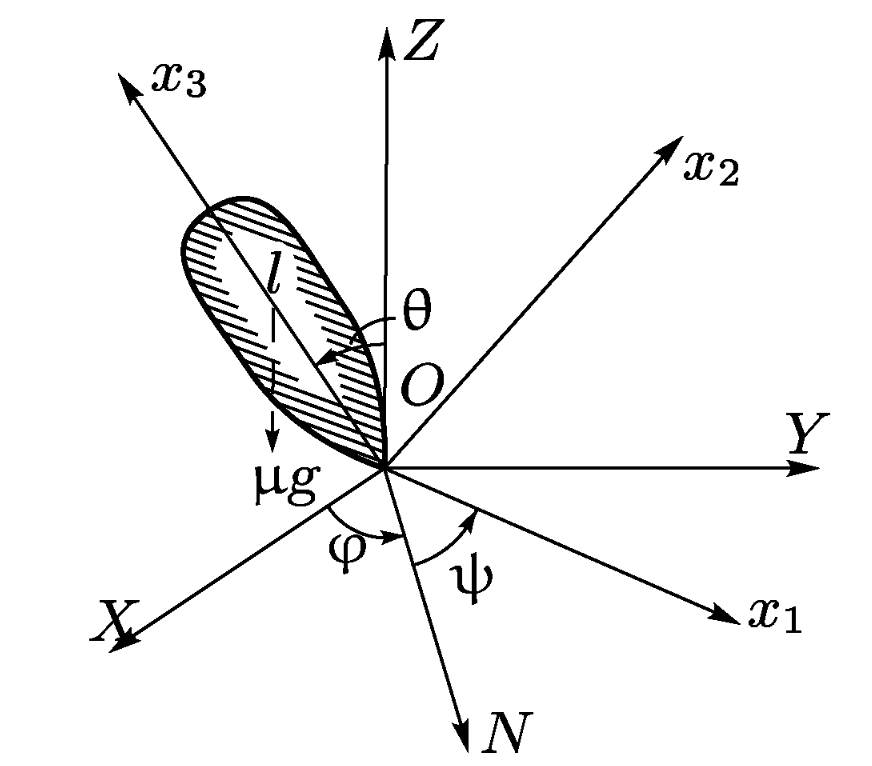
\includegraphics[width=0.25\textwidth]{figures/LL1.png}
    \caption{К задаче 11.72}
    %\label{fig:}
\end{figure}

